\documentclass[a4paper, oneside]{discothesis}

\usepackage[utf8]{inputenc}
\usepackage[T1]{fontenc}

%%%%%%%%%%%%%%%%%%%%%%%%%%%%%%%%%%%%%%%%%%%%%%%%%%%%%%%%%%%%%%%%%%%%%%%%%%%%%%%%%%%%%%%%%%%%%%%%%
% DOCUMENT METADATA

\thesistype{Semester Thesis} % Master's Thesis, Bachelor's Thesis, Semester Thesis, Group Project
\title{Asynchronous Consensus-Free Transaction Systems}

\author{Shoma Mori}
\email{shmori@student.ethz.ch}

\institute{Distributed Computing Group \\[2pt]
Computer Engineering and Networks Laboratory \\[2pt]
ETH Zürich}

% Optionally, you can put in your own logo here
%\logo{
\includegraphics[width=0.2\columnwidth]{figures/disco_logo_faded}}

\supervisors{Roland Schmid, Jakub Sliwinski\\[2pt] Prof.\ Dr.\ Roger Wattenhofer}

% Optionally, keywords and categories of the work can be shown (on the Abstract page)
%\keywords{Keywords go here.}
%\categories{ACM categories go here.}

\date{\today}

%%%%%%%%%%%%%%%%%%%%%%%%%%%%%%%%%%%%%%%%%%%%%%%%%%%%%%%%%%%%%%%%%%%%%%%%%%%%%%%%%%%%%%%%%%%%%%%%%

\begin{document}

\frontmatter % do not remove this line
\maketitle

\cleardoublepage

\begin{acknowledgements}
	I thank Lorem ipsum dolor sit amet, consetetur sadipscing elitr, sed diam nonumy eirmod tempor invidunt ut labore et dolore magna aliquyam erat, sed diam voluptua. At vero eos et accusam et justo duo dolores et ea rebum. Stet clita kasd gubergren, no sea takimata sanctus est Lorem ipsum dolor sit amet. Lorem ipsum dolor sit amet, consetetur sadipscing elitr, sed diam nonumy eirmod tempor invidunt ut labore et dolore magna aliquyam erat, sed diam voluptua. At vero eos et accusam et justo duo dolores et ea rebum. Stet clita kasd gubergren, no sea takimata sanctus est Lorem ipsum dolor sit amet.
\end{acknowledgements}


\begin{abstract}
    The abstract should be short, stating what you did and what the most important result is.
	Lorem ipsum dolor sit amet, consetetur sadipscing elitr, sed diam nonumy eirmod tempor invidunt ut labore et dolore magna aliquyam erat, sed diam voluptua. At vero eos et accusam et justo duo dolores et ea rebum. Stet clita kasd gubergren, no sea takimata sanctus est Lorem ipsum dolor sit amet. Lorem ipsum dolor sit amet, consetetur sadipscing elitr, sed diam nonumy eirmod tempor invidunt ut labore et dolore magna aliquyam erat, sed diam voluptua. At vero eos et accusam et justo duo dolores et ea rebum. Stet clita kasd gubergren, no sea takimata sanctus est Lorem ipsum dolor sit amet.
\end{abstract}

\tableofcontents

\mainmatter % do not remove this line

% Start writing here
\chapter{Introduction}

In the existing blockchain systems, it is assumed that the consensus problems
should be solved to achieve correctness.
For instance, Bitcoin uses proof-of-work to get consensus among agents in distributed systems.

However, proof-of-work algorithm takes much cost and therefore prevents scalability.
The transaction systems can get popularity if they get scalability improvement.

We introduce Asynchronous Consensus-Free Transaction Systems (ACFTS) aiming to get scalability
by removing consensus protocol.
ACFTS verifies transactions using agents call servers, which dedicate to manage transactions
and keep correctness in the system.
The servers put their signatures to prove the correctness of transactions.
Importantly, the servers work asynchronously meaning each server does not have to
communicate with other servers.
In other words, ACFTS does not need consensus.

We implemented ACFTS as a payment system and evaluated the throughput.
From the results, we found that the part of the verification of signatures becomes a bottleneck.

\chapter{Asynchronous Consensus-Free Transaction Systems}

\section{Model}
ACFTS consists of two kinds of agents called servers and clients.
The clients can send cryptocurrency to the other clients or themselves.
In the system, a transaction represents a transfer of cryptocurrency between clients.
Each client holds private and public key pairs
and the public keys are also called addresses, which are used to show owners of transactions.
The servers verify transactions when they receive them from clients
and record the history of valid transactions in their local storage.

Every client can send messages to all servers and all other clients.
In the same way, every server can send messages to all clients.
However, the servers do not send messages to the other servers.
Messages are delivered asynchronously, that is, messages reach to receivers eventually,
however, there is no guarantee that the messages arrive within finite time.


\section{Protocol}

\subsection{Transaciton}
A transaction represents a transfer of cryptocurrency from one client to other clients or itself.
Each transaction consists of one or more inputs and one or more outputs.

An input includes one or more outputs that will be spent.
The outputs which can be used as elements of inputs is called UTXO (Unspent Transaction Output).
Also, the input has a signature that is generated by a private key
corresponding to the public key (i.e. address) of the owner of the outputs.
Each UTXO can be spent by only the client who knows the private key
which is linked to the public key.

An output includes an address of its owner, amount of cryptocurrency, signatures from servers,
and a hash of outputs of the previous transaction.
In other words, transactions form a directed acyclic graph (DAG).
The sum of the amounts of outputs must be the same as one of the amounts of inputs.

In the case where a transaction has more than one output, the outputs have "siblings."
Each output is assigned an index in the siblings.
Normally, outputs can be identified with an address and the previous hash.
However, even if one transaction has multiple outputs that belong to the same addresses
and have the same previous transaction, they are identified by the indexes.

% TODO: insert graphs to describe the structure of transactions

\subsubsection{Genesis}
All outputs are created from any inputs, but the only genesis is different.
The genesis is an initial output and all outputs refer to the genesis as an ancestor.
The genesis is created by the system, its address represents the first owner
and the amount equals to the sum of the cryptocurrency.

\subsection{Server}
A server is a validator who has the role of verifying transactions from clients.
Every server records all transactions they verified in their memories.
When a server receives a transaction, firstly, the server checks
whether the outputs of the received transaction have been used in the past.
If even one of them has been used, the transaction is regarded to be invalid
and the server sends an error to the client.
If it is valid, nextly, the server verifies a client's signature to confirm the ownership.
Then, the server verifies signatures of servers which are also contained in the inputs.
We assume that each server knows the public keys of all the other servers.
Importantly, the number of valid signatures must be more than two-thirds of all servers
(the details will be described in ) to use the UTXOs. % FIXME: add ref
Finally, the server checks if the sum of the amounts of the outputs is the same
as one of the amounts of the inputs.
When the server completes the verification process without any errors,
it makes an own signature from the hash of the outputs using a private key of the server
and attaches it to the response to the client.
The number of signatures of one server for each transaction is only one,
which means the signature is created from the entire outputs, not from each output.
This reduces the number of necessary signatures and saves the cost as a result.
Finally, the server adds the outputs into their storage
and updates the status of the inputs to record that they cannot be used anymore.


\subsection{Client}
Clients can create new transactions.
They send requests for getting signatures from servers to make the transaction valid.
The client manages not only their own outputs but also their sibling outputs
because servers make a signature from the entire outputs in each transaction.
Therefore, the client needs to send the UTXOs with the siblings
in order to make it possible for servers to verify them.
The client attaches a signature to claim the ownership of the UTXOs when sending the request.

Consider a transfer of cryptocurrency from client $c_1$ to client $c_2$.
First, $c_1$ sends a request for the transaction to all servers and waits for the responses.
When $c_1$ gets signatures from more than two-thirds of all servers,
$c_1$ can "spend" the transaction.
In order to show the use of the UTXOs and make it possible for $c_2$ to use the new outputs,
$c_1$ sends $c_2$ the outputs with signatures of servers.
$c_2$ can confirm the transaction by verifying the signatures.

\subsection{The flow of a payment}
In our system, a payment is represented by a verified transaction.
The following is a flow of making a payment from client $c_1$ to $c_2$.

\begin{enumerate}
    \item $c_1$ finds UTXOs which $c_1$ has ownership of in their local storage.
    \item $c_1$ creates a request for a transaction whose output address is owned by $c_2$
        using the UTXOs including a $c_1$'s signature.
    \item $c_1$ sends the request to all servers and waits for the responses.
    \item Servers verify the transaction in the request.
    \item If the transaction has no errors, servers create their signatures and send them back
        as responses.
    \item When $c_1$ gets signatures from more than two-thirds of all servers,
        $c_1$ sends the output of the new transaction to $c_2$.
    \item When $c_2$ receives the output, $c_2$ verifies the signatures of servers.
    \item If the number of valid signatures is more than two-thirds of the number of all servers,
        the transaction is approved.
\end{enumerate}


\subsection{Double-spending}
In general transaction systems, using the same outputs more than twice,
namely, double-spending, is one of the main problems.
In our system, it is impossible to make conflicting valid transactions.

Consider a situation where $c_1$ tries to make two conflicting transactions
which are payments to $c_2$ and $c_3$.
To make a transaction valid, $c_1$ has to get signatures
from more than two-thirds of all servers.
However, if a server receives two conflicting transactions, it creates a signature for only one
transaction which comes first.
In other words, there are no ways to get signatures of both transactions from the same server.
Furthermore, it is not possible to send each transction to more than two-thirds of all servers
without overlapping.
In short, the two conflicting transactions can never be valid at the same time.

In this case, only one or neither transaction is confirmed.


\chapter{Implementation}
In this chapter, we describe the system in terms of implementation.

\section{Structure}
Servers and clients can communicate through the HTTP protocol.
Clients can send HTTP requests with JSON format.
Servers keep waiting for HTTP requests from clients.
Also, clients can make communication through the HTTP protocol
to receive UTXOs which are related to themselves.
Therefore, clients also keep waiting for HTTP requests at the same time
as making requests of new transactions.

Both servers and clients have their database to record transaction outputs.

Genesis is initially recorded in a client that has the genesis and all servers.

\section{Documentations}

\subsection{Signature}
ACFTS uses public key cryptography to show ownership of outputs and completion of verification.
The implementation adopts the Elliptic Curve Digital Signature Algorithm (ECDSA)
for key pairs and verification processes.

Clients create a hash of UTXOs with SHA256 and sign on it with a private key
which is generated with ECDSA when creating a new transaction.
Servers verify the signature with the public key of clients and sign on the UTXOs
with a private key of the servers.
The receiver of the transaction can verify the signatures of servers with public keys
of servers.

\subsubsection{UTXO hash}
A UTXO have an address, a hash of outputs of the previous transaction and an index of siblings.
We can show that UTXOs can be identified with these keys.

% FIXME: もっとわかりやすく説明する
Hash values become the same deterministically if the inputs are the identical.
The input of the hash includes a hash of two transactions ago.
In other words, every hash of outputs has information of all transactions
which precedes the outputs.
From the genesis, each output has an index even if the previous transaction is the same.
Therefore, every output has diffrent hash values without collisions of the hash function.


\subsection{Change transaction}
When a client tries to create a request for a transaction,
the client finds UTXOs until the sum of the amounts
becomes larger than the amount the client wants to send.
If the sum exceeds the expected amount, the clients make a change transaction
to make both ends meet.

\subsection{Cluster}
In the implementation, multiple client addresses can be managed in one database.
We call the set of addresses cluster.
When creating transactions among one cluster, it is not necessary to send UTXOs
because they can refer to through the shared memory.
In some sense, a cluster is a wallet and transactions in one cluster represent sorting out UTXOs.
When creating transactions among different clusters, it is required to send the UTXOs,
which is a real payment.

In the initialization process, each cluster exchange their addresses
and therefore can decide to which cluster they should send UTXOs when creating new transactions.


\chapter{Experiment}
We evaluated the throughputs of our systems by experiments using some scenarios of transactions.
The system is implemented in Go and was benchmarked in a local environment.
We do not assume network delay.

We also profiled the system to find bottlenecks aiming for improving the throughputs.

\section{Environments}
\begin{itemize}
    \item The number of servers: 4
    \item The number of clusters: 2 ($cs0$ and $cs1$)
    \item The number of clients in each cluseter: 4\\
        ($\{ct0, ct1, ct2, ct3\} \in cs0$ and $\{ct4, ct5, ct6, ct7\} \in cs1$)
    \item The genesis: $amount = 1000000$, $owner = cs0$
\end{itemize}

We executed the following five diffrent scenarios.
Every arrow indicates transfer of one amount of cryptocurrency.
\begin{itemize}
    \item Scenario1: $ct0 \rightarrow ct1$
    \item Scenario2: $ct0 \rightarrow ct1$, $ct1 \rightarrow ct0$
    \item Scenario3: $ct0 \rightarrow ct1$, $ct1 \rightarrow ct0$, $ct2 \rightarrow ct3$, $ct3 \rightarrow ct2$
    \item Scenario4: $random \rightarrow random~(rondom \in cs0)$
    \item Scenario5: $ct0 \rightarrow ct4$
\end{itemize}
Note that sender and receiver are chosen from $cs0$ with equal probability in scenario4.

\section{Results}

\subsection{Processing speed}
Trials in tables means that execution of a set of transctions in one scenario counts one trial.
For example, in scenario1, when trials is 10, transfer from $ct0$ to $ct1$ is executed 10 times.
On the other hand, in scenario2, when when trials is 10, transfers from $ct0$ to $ct1$
and $ct1$ to $ct0$ are executed 10 times respectively.
Speed is the number of approved transactions per second.

\begin{table}[htb]
    \begin{center}
        \begin{tabular}{c}

            \begin{minipage}{0.5\hsize}
                \begin{center}
                    \caption{Scenario1}
                    \begin{tabular}{|l|c|} \hline
                        trials [tx] & speed [tx/s]\\ \hline \hline
                        10 & 4.30 \\
                        100 & 5.25 \\
                        1000 & 4.37 \\ 
                        10000 & 3.10 \\ \hline
                    \end{tabular}
                \end{center}
            \end{minipage}

            \begin{minipage}{0.5\hsize}
                \begin{center}
                    \caption{Scenario2}
                    \begin{tabular}{|l|c|} \hline
                        trials [tx] & speed [tx/s]\\ \hline \hline
                        10 & 5.11 \\
                        100 & 5.56 \\
                        1000 & 4.82 \\
                        10000 & 1.52 \\ \hline
                    \end{tabular}
                \end{center}
            \end{minipage}

        \end{tabular}
    \end{center}
\end{table}


\begin{table}[htbp]
    \begin{center}
        \begin{tabular}{c}

            \begin{minipage}{0.5\hsize}
                \begin{center}
                    \caption{Scenario3}
                    \begin{tabular}{|l|c|} \hline
                        trials [tx] & speed [tx/s]\\ \hline \hline
                        10 & 5.35 \\
                        100 & 5.51 \\
                        1000 & 5.06 \\
                        10000 & 1.98 \\ \hline
                    \end{tabular}
                \end{center}
            \end{minipage}

            \begin{minipage}{0.5\hsize}
                \begin{center}
                    \caption{Scenario4}
                    \begin{tabular}{|l|c|} \hline
                        trials [tx] & speed [tx/s]\\ \hline \hline
                        10 & 5.13 \\
                        100 & 4.40 \\
                        1000 & 5.13 \\
                        10000 & 1.97  \\ \hline
                    \end{tabular}
                \end{center}
            \end{minipage}

        \end{tabular}
    \end{center}
\end{table}

\begin{table}[htb]
  \begin{center}
    \caption{Scenario5}
    \begin{tabular}{|l|c|} \hline
        trials [tx] & speed [tx/s]\\ \hline \hline
        10 & 3.10 \\
        100 & 3.13 \\
        1000 & 4.54 \\
        10000 & 2.52 \\ \hline
    \end{tabular}
  \end{center}
\end{table}

There are some points that can observe from each table.
Although there is an exemption, in the most scenarios, the throughput improves
when trials goes from 10tx to 100tx.
After that, although there is an exemption too, the throughputs go down as incresing
the number of transacitons.
Especially, the throughputs become less than half when trials go from 1000tx to 10000tx
in some scenarios.

Next, we can get some tendencies when comparing diffrent scenarios.
From scenario1 to 4 are sets of transactions in one cluster,
but scenario5 is a set of ones between two clusters.
The overall throughput of scenario5 is less than the others.

% TODO: Scenario間で10000のときなど,throughputが異なる理由を考える


\subsection{Bottlenecks}
We employed flame graphs to find bottlenecks of the system.

\subsubsection{Flame graph}
Flame graph is a visualization tool which allows identify the most frequent code-paths.
The y-axis shows the stack depth, ordered from root at the top to leaf at the bottom.
The x-axis spans the stack trace collection.
The width of each function box shows the frequency at which that function was present
in the stack traces, or part of a stack trace ancestry.
Bottleneck functions have wide width boxes in the flame graphs.

% TODO: どんなtxを実行しているときに記録したflame graphなのかに言及する
% TODO: txの数が増えているときのflame graphも載せる

\begin{figure}
    \begin{center}
        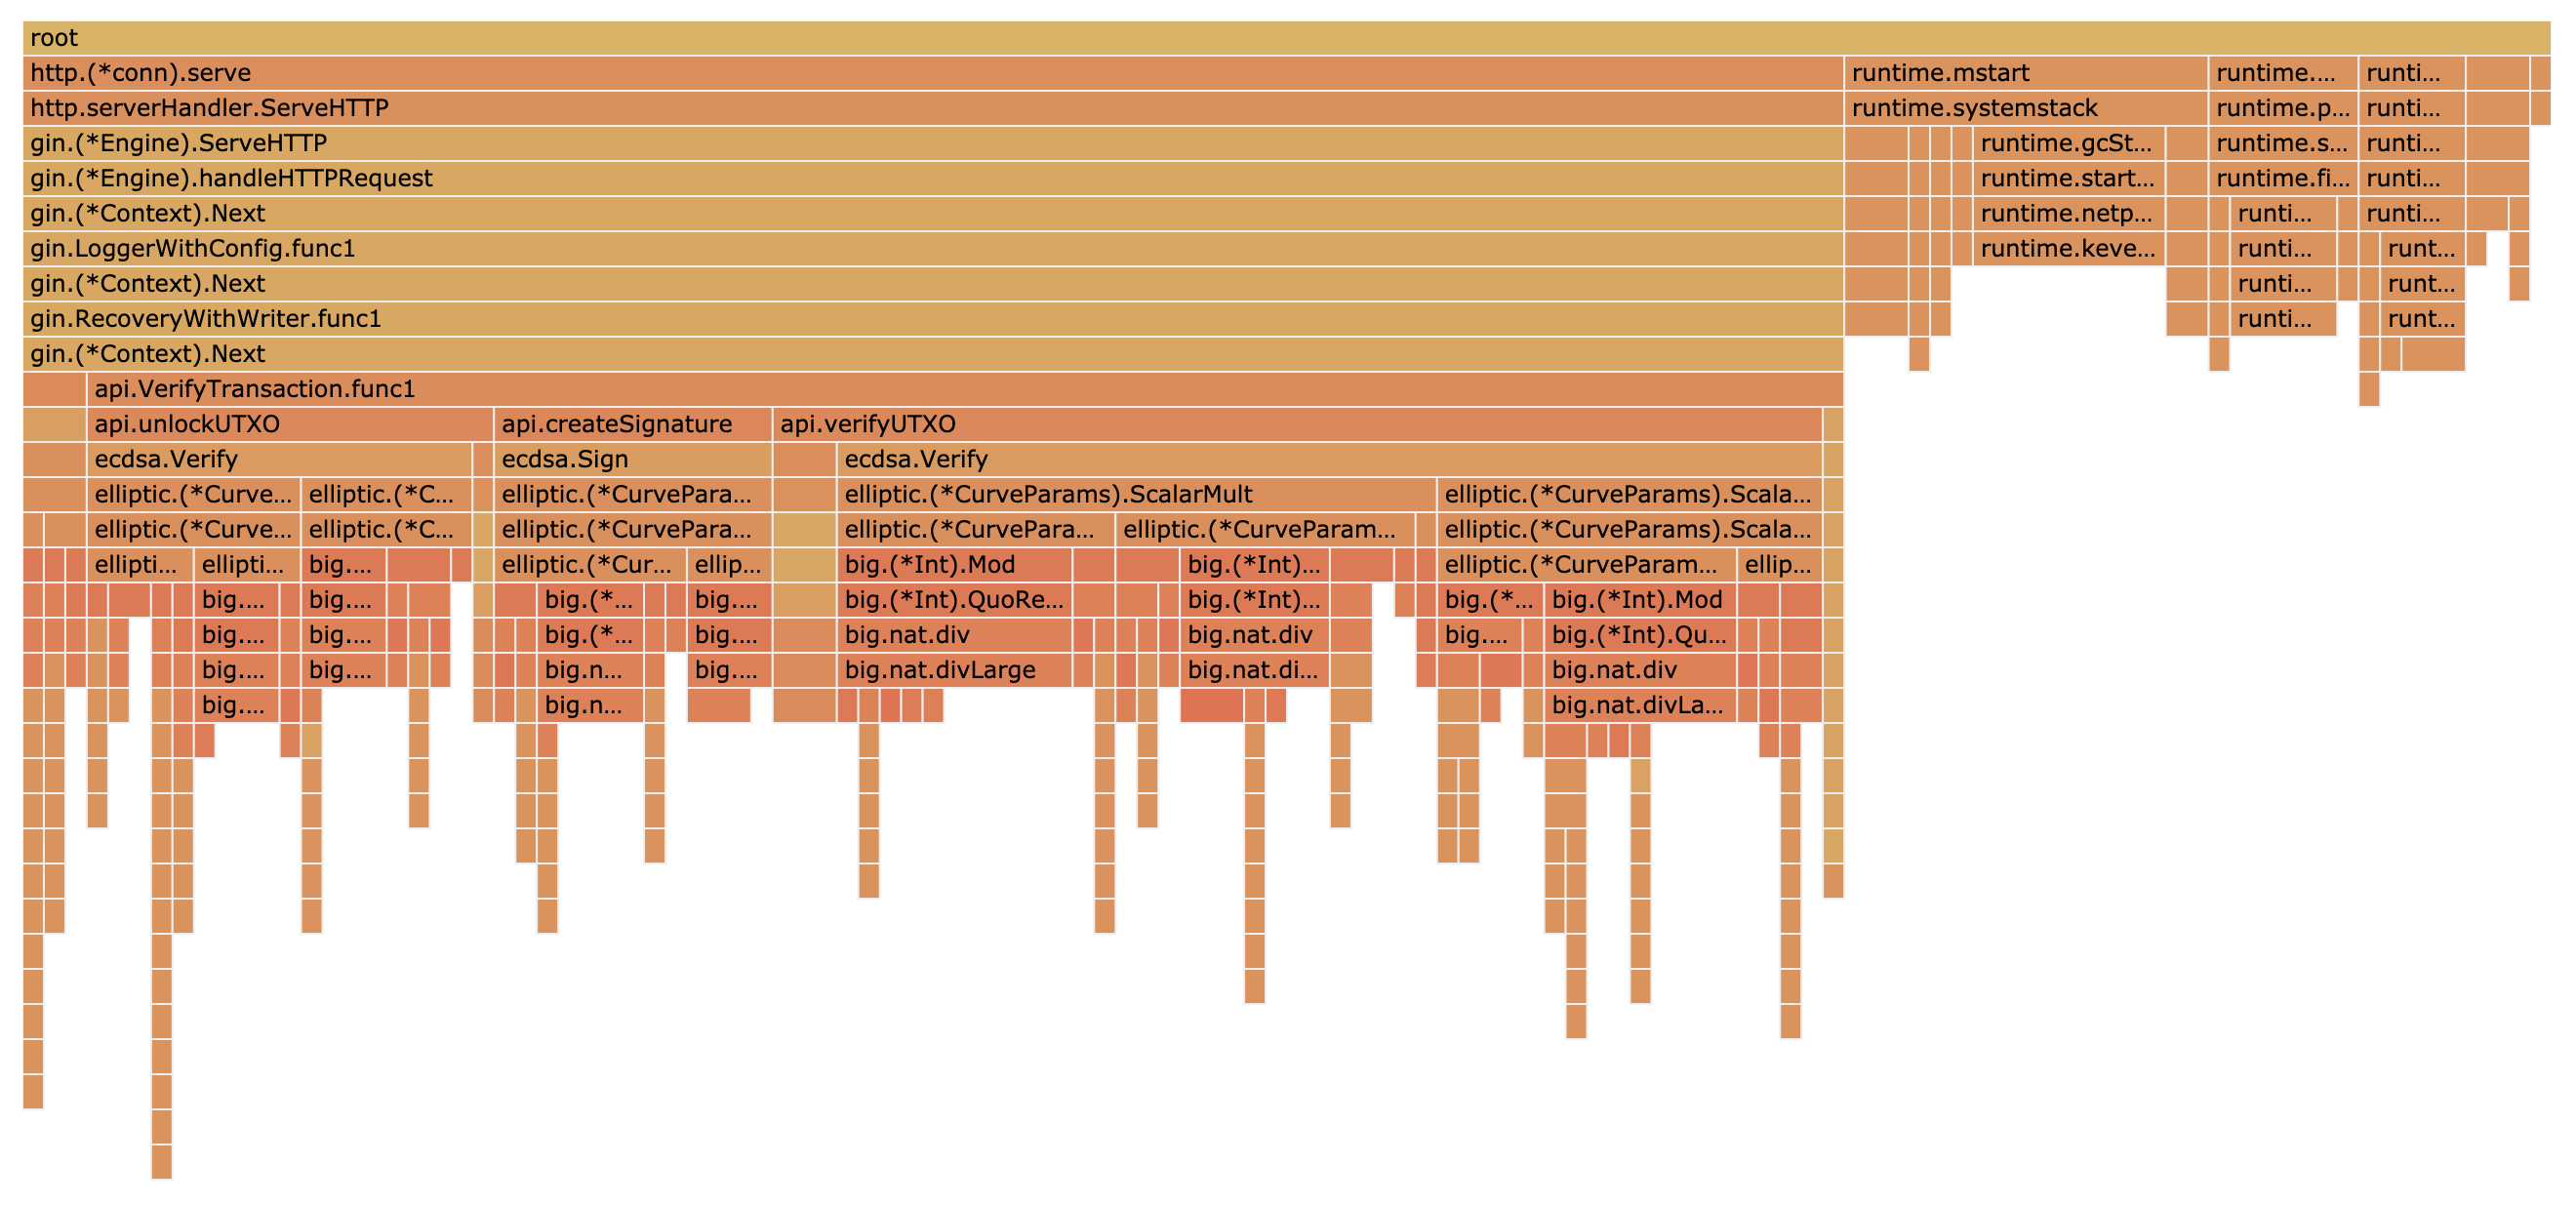
\includegraphics[width=\columnwidth]{figures/server_flame_graph}
        \caption{Flame graph in a server}
        \label{fig:server-fg}
    \end{center}
\end{figure}

\begin{figure}
    \begin{center}
        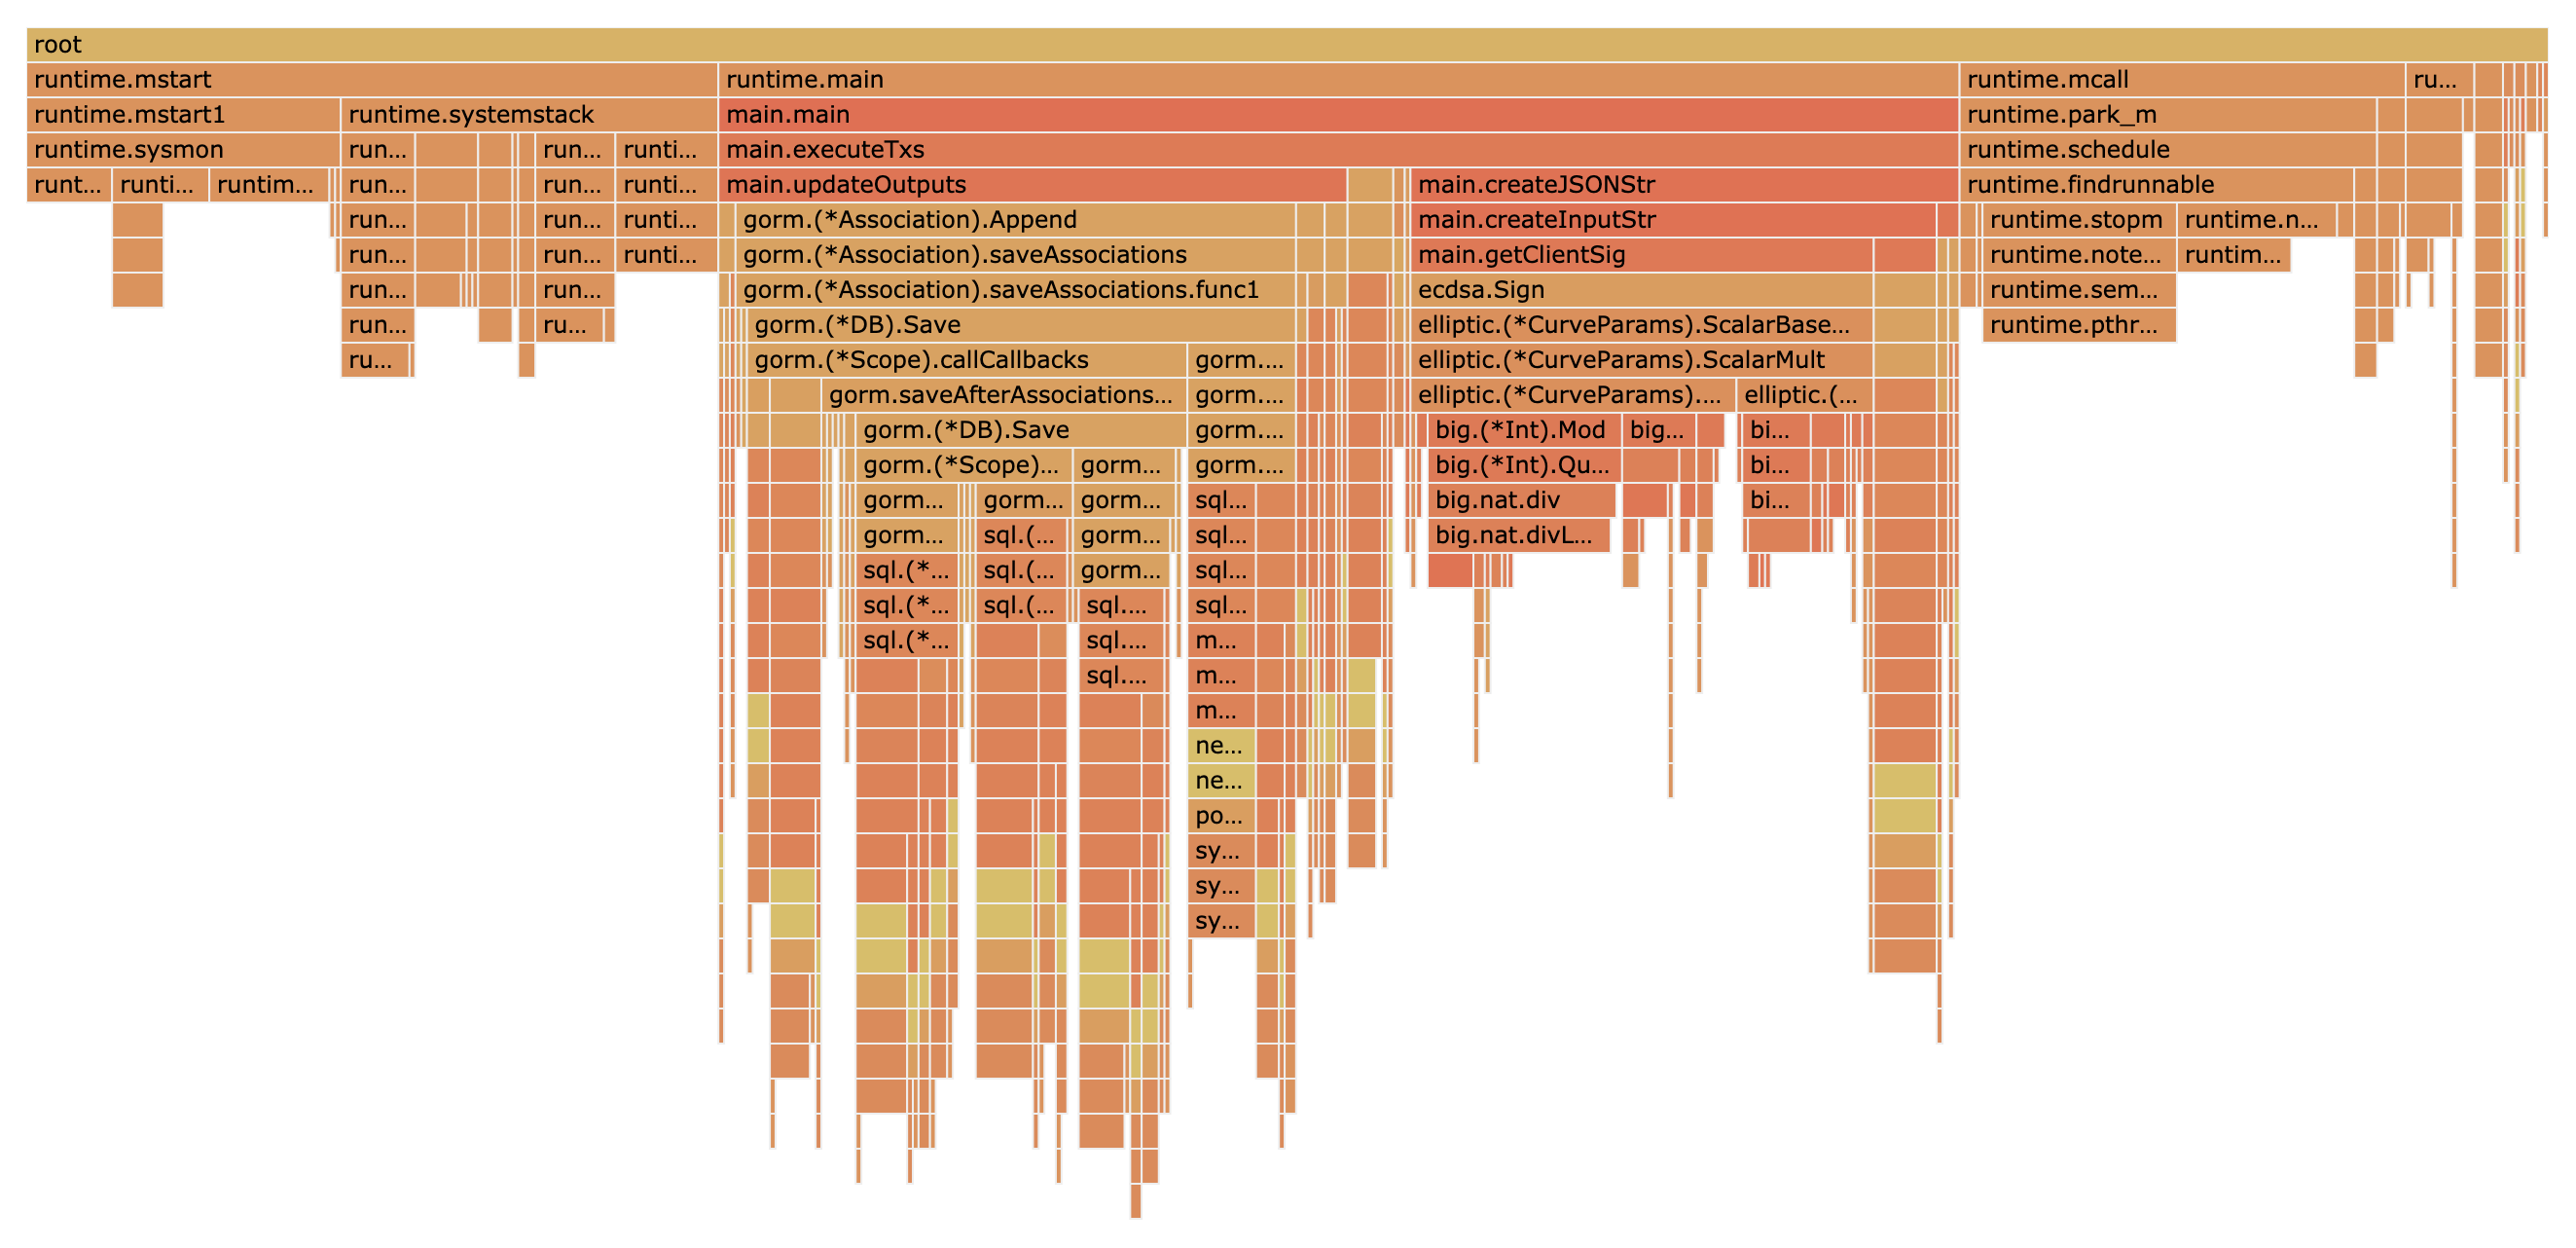
\includegraphics[width=\columnwidth]{figures/client_flame_graph}
        \caption{Flame graph in a client}
        \label{fig:client-fg}
    \end{center}
\end{figure}

As we can see in the flame graph of a server-side, % FIXME: insert ref
it is found that api.verifyUTXO, api.unlockUTXO and api.createSignature cost much.
If you trace the stacks, ecdsa.Verify and ecdsa.Sign are the causes of the bottlenecks.
ecdsa is a cryptographic library of the Elliptic Curve Digital Signature Algorithm in Go.
In api.verifyUTXO, a server verifies signatures of the receiving UTXO used in the inputs.
In api.unlockUTXO, a server verifies a signature of the client who sent the request.
In api.createSignature, a server issue a signature to prove the correctness of the transaction.

\section{Discussion}
% TODO: why the throughput goes up from 10x to 100x

% TODO: why the throughput goes down from 1000x to 10000x

\subsection{Transaction between different clusters}
Throughput of scenario5 is smaller than the other scenarios.
Clients have to send UTXOs to different clusters
when they make outputs that include ones belonging to different clusters.
Now the sender waits for a response from the receiver, which can cost time.

One of the ways to improve throughputs of transactions among clusters
is that not to wait for the responses.
Actually, in the real use of this system such as payment in cafe,
a payer sends signatures of servers in some way or just show something (e.g. QR code)
which has the information.
Then, it is not necessary for a payee to respond in some digital way.


% TODO: how to remove (reduce) the bottlenecks
\subsection{Waiting for signatures from servers}
Currently, clients wait for responses from all servers
after they sent requests of new transactions.
However, it is enought if they have only two-thirds of all signatures
to show the validity of the new transactions.
Suppose that a client sends valid transaction and all servers will send signatures back,
if the client do not wait after getting more than two-thirds of all signatures,
the speed will 1.5 times faster.


\subsection{Algorithm for cryptographic processes}
The most of bottlenecks is attributed to crytographic processes
such as make signatures and verification of the signatures.
There are no specific reasons why we must adopt ECDSA as the algorithm
for the cryptographic processes.
We can take into account other algorithms for our system.


\subsection{Changes of servers}
Now the number of servers and their addresses are fixed.
However, if the servers are fixed permanetly,
they can be a vulnerability when some of them stop or break.
To avoid that situation, the system should adapt to changes of servers.

\subsection{Run in a real environment}
% TODO: write about real environments like AWS

\chapter{Conclusion}
foofoofoofoofoofoofoofoofoofoofoofoofoofoofoofoofoofoofoofoofoofoo
\TODO{This is a TODO annotation.}

\begin{theorem}[First Theorem] \label{thm:first theorem}
	This is our first theorem.
\end{theorem}

\begin{proof}
	And this is the proof of the first theorem with a complicated formula and a reference to Theorem \ref{thm:first theorem}. Lorem ipsum dolor sit amet, consetetur sadipscing elitr, sed diam nonumy eirmod tempor invidunt ut labore et dolore magna aliquyam erat, sed diam voluptua. Lorem ipsum dolor sit amet, consetetur sadipscing elitr, sed diam nonumy eirmod tempor invidunt ut labore et dolore magna aliquyam erat, sed diam voluptua.
	\begin{equation}
		{\frac {\mathrm d}{\mathrm dx}}\arctan(\sin({x}^{2}))=-2 \cdot {\frac {\cos({x}^{2})x}{-2+\left (\cos({x}^{2})\right )^{2}}}
	\end{equation}
\end{proof}

\begin{figure}
    \centering
    
\includegraphics[width=0.2\columnwidth]{figures/disco_logo_faded}
    \caption{This is an example graphic.}
    \label{fig:example_figure}
\end{figure}

And here we cite some external documents~\cite{TestReference, TestReference2}.
An example of an included graphic can be found in Figure~\ref{fig:example_figure}.
Note that in \LaTeX, ``quotes'' do not use the usual double quote characters.

% This displays the bibliography for all cited external documents. All references have to be defined in the file references.bib and can then be cited from within this document.
\bibliographystyle{IEEEtran}
\bibliography{references}

% This creates an appendix chapter, comment if not needed.
\appendix
\chapter{First Appendix Chapter Title}

\end{document}
